\documentclass[11pt,a4paper]{article}
\usepackage[margin=1.9cm, top=2.1cm, bottom=2.0cm]{geometry}
\usepackage[T1]{fontenc}
\usepackage{lmodern}
\usepackage{amsmath,amssymb}
\usepackage{enumitem,booktabs,array,tabularx,multirow}
\usepackage[normalem]{ulem}
\usepackage{adjustbox}
\usepackage{xcolor}
\usepackage{fancyhdr,lastpage}
\usepackage[most]{tcolorbox}
\usepackage{tikz}
\usetikzlibrary{shapes.geometric,arrows.meta,positioning,calc}
\usepackage[hidelinks]{hyperref}
\setlength{\parindent}{0pt}
\setlength{\parskip}{4pt}
\renewcommand{\arraystretch}{1.25}
\emergencystretch=2em
\pagestyle{fancy}\fancyhf{}
\lhead{\small\textit{Course: CS420 -- Artificial Intelligence}}
\rhead{\small Practice Test 3}
\cfoot{\small Page \thepage\ of \pageref{LastPage}}
\renewcommand{\headrulewidth}{0.4pt}
% empty answer box (exam) / filled box (solution)
\newtcolorbox{ansbox}[1][]{enhanced, breakable, colback=white, colframe=black!55, boxrule=0.5pt, arc=0pt,
  left=5pt, right=5pt, top=3pt, bottom=3pt, before skip=3pt, after skip=6pt, #1}
\newtcolorbox{solbox}{enhanced, breakable, colback=blue!2!white, colframe=blue!50!black, boxrule=0.6pt, arc=0pt,
  left=6pt, right=6pt, top=4pt, bottom=4pt, before skip=3pt, after skip=8pt,
  fontupper=\color{black}}
\newcommand{\question}[1]{\par\medskip\noindent\textbf{Question #1.}\ }
\newcommand{\subq}[1]{\par\smallskip\noindent\textbf{#1}\ }
\newcommand{\T}{\textbf{\textcolor{green!45!black}{TRUE}}}
\newcommand{\F}{\textbf{\textcolor{red!70!black}{FALSE}}}

\tikzset{
  maxn/.style={draw, thick, regular polygon, regular polygon sides=3, minimum size=10.5mm, inner sep=0pt, font=\small},
  minn/.style={maxn, shape border rotate=180},
  chn/.style={draw, thick, circle, minimum size=9.5mm, inner sep=0pt, font=\small},
  leafn/.style={draw, rectangle, minimum width=5.5mm, minimum height=5.5mm, inner sep=1pt, font=\small},
  gone/.style={draw=black!25, text=black!35},
  cut/.style={red!80!black, very thick, dashed},
  sol/.style={text=blue!70!black, font=\small\bfseries},
}

\begin{document}


{\large\textbf{\textit{Course: CS420 -- Artificial Intelligence}}}\par
{\textbf{\textit{Midterm examination review -- Lectures 0 to 3}}}\par
\begin{center}{\Large\bfseries PRACTICE MIDTERM EXAMINATION -- TEST 3}\\[3pt]
{\small Duration: 120 minutes \quad$\cdot$\quad Closed book \quad$\cdot$\quad Calculator allowed}\end{center}
\noindent\rule{\linewidth}{0.6pt}

\noindent Full name: \rule{6.5cm}{0.3pt}\hfill Student ID: \rule{4cm}{0.3pt}\par\smallskip
{\small\textit{Unless a question says otherwise, ties are broken in alphabetical order (left-to-right in trees), and successors are generated in alphabetical order.}}\par
\question{1}\textit{Tower of Hanoi with 3 pegs and 3 disks.} Three disks of different sizes are stacked on peg 1 (largest at the bottom). The goal is to move the stack to peg 3, moving one disk at a time and never placing a larger disk on a smaller one.
\subq{(a)}Consider a state as a tuple of values. Which values should be included in the tuple?
\begin{ansbox}[height=1.0cm]\end{ansbox}
\subq{(b)}Define the initial state and the goal state.
\begin{ansbox}[height=0.8cm]\end{ansbox}
\subq{(c)}Define the action function.
\begin{ansbox}[height=1.5cm]\end{ansbox}
\subq{(d)}What is the action cost?
\begin{ansbox}[height=0.6cm]\end{ansbox}
\subq{(e)}What is the maximum number of states? How many are reachable? What is the length of an optimal solution?
\begin{ansbox}[height=1.2cm]\end{ansbox}
\question{2}Consider the undirected graph below; $S$ is the initial state and $G$ the goal state. \begin{center}
\begin{adjustbox}{max width=\linewidth}
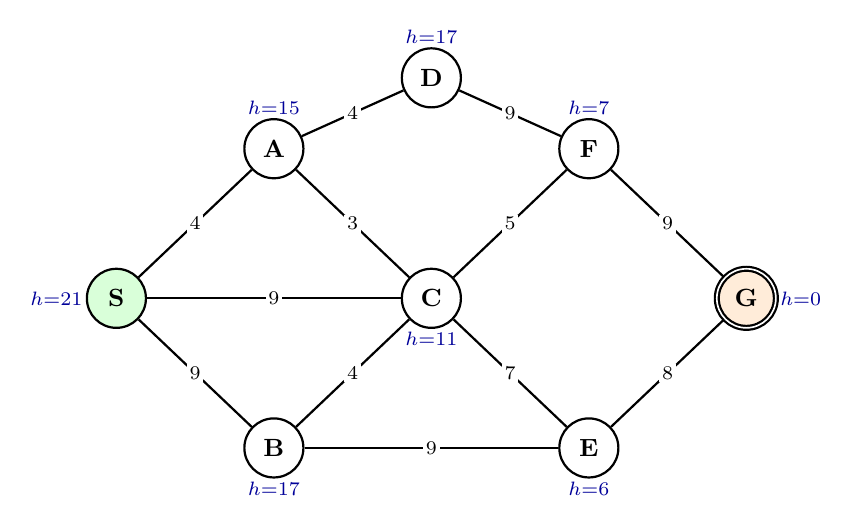
\begin{tikzpicture}[scale=1.0, every node/.style={transform shape}, gn/.style={draw, thick, circle, minimum size=7.5mm, inner sep=0pt, font=\small\bfseries}, ec/.style={font=\scriptsize, fill=white, inner sep=1pt}]
\node[gn, fill=green!15, label={[font=\scriptsize, text=blue!60!black, inner sep=1pt]left:$h{=}21$}] (S) at (0.00,0.00) {S};
\node[gn, label={[font=\scriptsize, text=blue!60!black, inner sep=1pt]above:$h{=}15$}] (A) at (2.00,1.90) {A};
\node[gn, label={[font=\scriptsize, text=blue!60!black, inner sep=1pt]below:$h{=}17$}] (B) at (2.00,-1.90) {B};
\node[gn, label={[font=\scriptsize, text=blue!60!black, inner sep=1pt]below:$h{=}11$}] (C) at (4.00,0.00) {C};
\node[gn, label={[font=\scriptsize, text=blue!60!black, inner sep=1pt]above:$h{=}17$}] (D) at (4.00,2.80) {D};
\node[gn, label={[font=\scriptsize, text=blue!60!black, inner sep=1pt]below:$h{=}6$}] (E) at (6.00,-1.90) {E};
\node[gn, label={[font=\scriptsize, text=blue!60!black, inner sep=1pt]above:$h{=}7$}] (F) at (6.00,1.90) {F};
\node[gn, double, fill=orange!15, label={[font=\scriptsize, text=blue!60!black, inner sep=1pt]right:$h{=}0$}] (G) at (8.00,0.00) {G};
\draw[thick] (S) to[] node[ec, midway]{4} (A);
\draw[thick] (S) to[] node[ec, midway]{9} (B);
\draw[thick] (S) to[] node[ec, midway]{9} (C);
\draw[thick] (A) to[] node[ec, midway]{3} (C);
\draw[thick] (A) to[] node[ec, midway]{4} (D);
\draw[thick] (B) to[] node[ec, midway]{4} (C);
\draw[thick] (B) to[] node[ec, midway]{9} (E);
\draw[thick] (C) to[] node[ec, midway]{5} (F);
\draw[thick] (C) to[] node[ec, midway]{7} (E);
\draw[thick] (D) to[] node[ec, midway]{9} (F);
\draw[thick] (E) to[] node[ec, midway]{8} (G);
\draw[thick] (F) to[] node[ec, midway]{9} (G);
\end{tikzpicture}
\end{adjustbox}
\end{center}For each search strategy, (a) list, in order, the states \textbf{expanded}, (b) give the path found and (c) give the final content of the frontier (a state is expanded when it is removed from the frontier). Conventions: BFS, DFS and greedy best-first search test a state for the goal when it is \emph{generated} (so the goal is not expanded); UCS and A* test it when it is \emph{removed} from the frontier (graph search; a cheaper path to a frontier state replaces its entry). DFS avoids loops by remembering the states on the current path only. The path returned will not be accepted if the list of expanded states is wrong.

\begin{center}\small\begin{tabularx}{\linewidth}{|>{\raggedright}p{2.6cm}|>{\raggedright}X|>{\raggedright}p{3.6cm}|>{\raggedright\arraybackslash}p{2.6cm}|}\hline
\textbf{Algorithm} & \textbf{List of expanded states} & \textbf{Path returned} & \textbf{Final frontier}\\ \hline
Breadth-first search & & & \\[8mm] \hline
Uniform-cost search & & & \\[8mm] \hline
Depth-first search & & & \textit{(not asked)}\\[8mm] \hline
Greedy best-first search & & & \\[8mm] \hline
Graph-search A* & & & \\[8mm] \hline
\end{tabularx}\end{center}
\subq{(d)}Is $h$ admissible? Justify.
\begin{ansbox}[height=1.2cm]\end{ansbox}
\subq{(e)}Is $h$ consistent? List every violated inequality.
\begin{ansbox}[height=1.6cm]\end{ansbox}
\subq{(f)}Decrease as few $h$-values as possible so that $h$ becomes consistent. Does the new heuristic dominate the old one, or the opposite?
\begin{ansbox}[height=1.8cm]\end{ansbox}
\clearpage
\question{3}The 4-queens problem asks to place four queens on a $4\times4$ board so that no queen attacks another. States are configurations with all four queens on the board, one per column; a successor moves one queen to another square of its column; $h(\text{state})$ is the number of attacking pairs. The initial state $S$ (written as rows $1,1,1,1$; row 1 at the top) is shown below.\begin{center}
\begin{adjustbox}{max width=\linewidth}
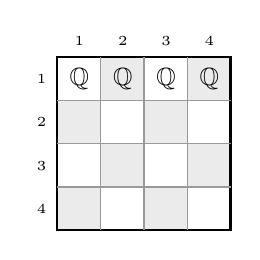
\begin{tikzpicture}
\fill[white] (0.00,0.00) rectangle +(0.55,-0.55);
\fill[black!8] (0.00,-0.55) rectangle +(0.55,-0.55);
\fill[white] (0.00,-1.10) rectangle +(0.55,-0.55);
\fill[black!8] (0.00,-1.65) rectangle +(0.55,-0.55);
\fill[black!8] (0.55,0.00) rectangle +(0.55,-0.55);
\fill[white] (0.55,-0.55) rectangle +(0.55,-0.55);
\fill[black!8] (0.55,-1.10) rectangle +(0.55,-0.55);
\fill[white] (0.55,-1.65) rectangle +(0.55,-0.55);
\fill[white] (1.10,0.00) rectangle +(0.55,-0.55);
\fill[black!8] (1.10,-0.55) rectangle +(0.55,-0.55);
\fill[white] (1.10,-1.10) rectangle +(0.55,-0.55);
\fill[black!8] (1.10,-1.65) rectangle +(0.55,-0.55);
\fill[black!8] (1.65,0.00) rectangle +(0.55,-0.55);
\fill[white] (1.65,-0.55) rectangle +(0.55,-0.55);
\fill[black!8] (1.65,-1.10) rectangle +(0.55,-0.55);
\fill[white] (1.65,-1.65) rectangle +(0.55,-0.55);
\draw[thick] (0,0) rectangle (2.20,-2.20);
\draw[black!40] (0.55,0) -- (0.55,-2.20);
\draw[black!40] (0,-0.55) -- (2.20,-0.55);
\draw[black!40] (1.10,0) -- (1.10,-2.20);
\draw[black!40] (0,-1.10) -- (2.20,-1.10);
\draw[black!40] (1.65,0) -- (1.65,-2.20);
\draw[black!40] (0,-1.65) -- (2.20,-1.65);
\node[font=\small\bfseries] at (0.28,-0.28) {$\mathbb{Q}$};
\node[font=\small\bfseries] at (0.83,-0.28) {$\mathbb{Q}$};
\node[font=\small\bfseries] at (1.38,-0.28) {$\mathbb{Q}$};
\node[font=\small\bfseries] at (1.93,-0.28) {$\mathbb{Q}$};
\node[font=\tiny] at (0.28,0.20) {1};
\node[font=\tiny] at (0.83,0.20) {2};
\node[font=\tiny] at (1.38,0.20) {3};
\node[font=\tiny] at (1.93,0.20) {4};
\node[font=\tiny] at (-0.20,-0.28) {1};
\node[font=\tiny] at (-0.20,-0.83) {2};
\node[font=\tiny] at (-0.20,-1.38) {3};
\node[font=\tiny] at (-0.20,-1.93) {4};
\end{tikzpicture}
\end{adjustbox}
\end{center}
\subq{(a)}How many states are there in total? How many successors does each state have? Explain.
\begin{ansbox}[height=1.0cm]\end{ansbox}
\subq{(b)}What is $h(S)$? Explain.
\begin{ansbox}[height=0.8cm]\end{ansbox}
\subq{(c)}Apply steepest-descent hill climbing from $S$. At every step write the $h$ value of each of the 12 successors on the board (in the square the queen would move to) and choose the best one (ties: left-most column, then top row). Stop at a solution or when no successor is better.
\begin{ansbox}[height=8.0cm]\end{ansbox}
\clearpage
\question{4}Consider the following 4-ply game tree (MAX at the root, children visited left to right).\begin{center}
\begin{adjustbox}{max width=\linewidth}
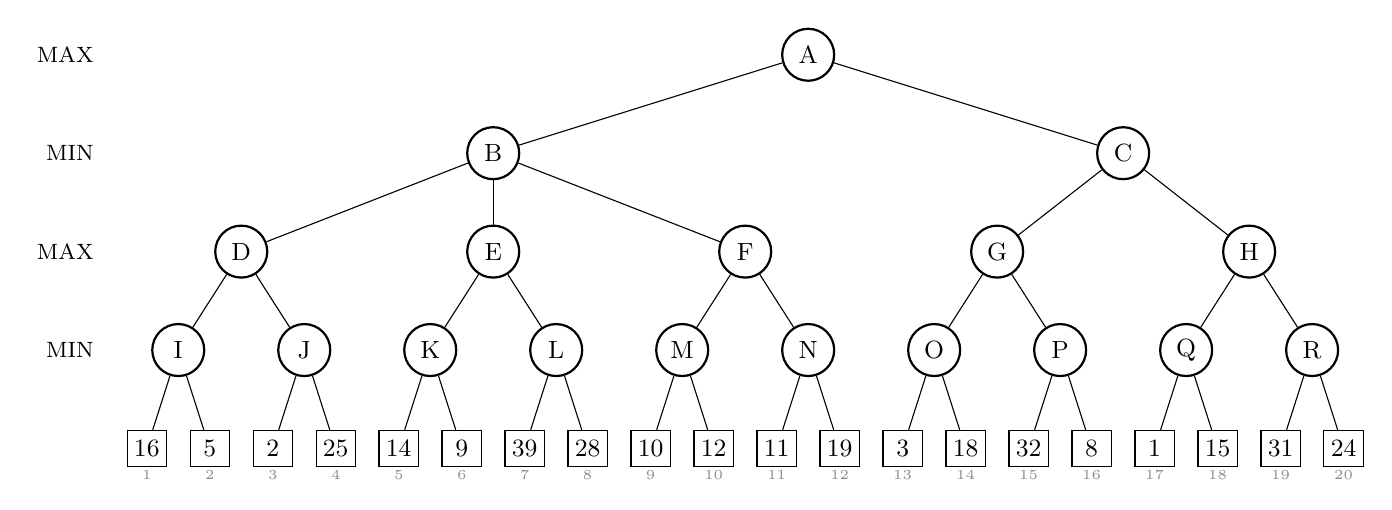
\begin{tikzpicture}[scale=1.0, every node/.style={transform shape}, gc/.style={draw, thick, circle, minimum size=6.6mm, inner sep=0pt, font=\small}, gl/.style={draw, rectangle, minimum width=5mm, minimum height=4.6mm, inner sep=1pt, font=\small}, gx/.style={draw=black!25, text=black!35}, val/.style={font=\footnotesize\bfseries, text=red!80!black, inner sep=1pt}]
\node[font=\footnotesize, anchor=east] at (-0.55,0.00) {MAX};
\node[font=\footnotesize, anchor=east] at (-0.55,-1.25) {MIN};
\node[font=\footnotesize, anchor=east] at (-0.55,-2.50) {MAX};
\node[font=\footnotesize, anchor=east] at (-0.55,-3.75) {MIN};
\node[gc] (n37) at (8.400,0.000) {A};
\node[gc] (n21) at (4.400,-1.250) {B};
\node[gc] (n6) at (1.200,-2.500) {D};
\node[gc] (n2) at (0.400,-3.750) {I};
\node[gl, label={[font=\tiny, text=black!45, inner sep=1pt]below:1}] (n0) at (0.000,-5.000) {16};
\node[gl, label={[font=\tiny, text=black!45, inner sep=1pt]below:2}] (n1) at (0.800,-5.000) {5};
\node[gc] (n5) at (2.000,-3.750) {J};
\node[gl, label={[font=\tiny, text=black!45, inner sep=1pt]below:3}] (n3) at (1.600,-5.000) {2};
\node[gl, label={[font=\tiny, text=black!45, inner sep=1pt]below:4}] (n4) at (2.400,-5.000) {25};
\node[gc] (n13) at (4.400,-2.500) {E};
\node[gc] (n9) at (3.600,-3.750) {K};
\node[gl, label={[font=\tiny, text=black!45, inner sep=1pt]below:5}] (n7) at (3.200,-5.000) {14};
\node[gl, label={[font=\tiny, text=black!45, inner sep=1pt]below:6}] (n8) at (4.000,-5.000) {9};
\node[gc] (n12) at (5.200,-3.750) {L};
\node[gl, label={[font=\tiny, text=black!45, inner sep=1pt]below:7}] (n10) at (4.800,-5.000) {39};
\node[gl, label={[font=\tiny, text=black!45, inner sep=1pt]below:8}] (n11) at (5.600,-5.000) {28};
\node[gc] (n20) at (7.600,-2.500) {F};
\node[gc] (n16) at (6.800,-3.750) {M};
\node[gl, label={[font=\tiny, text=black!45, inner sep=1pt]below:9}] (n14) at (6.400,-5.000) {10};
\node[gl, label={[font=\tiny, text=black!45, inner sep=1pt]below:10}] (n15) at (7.200,-5.000) {12};
\node[gc] (n19) at (8.400,-3.750) {N};
\node[gl, label={[font=\tiny, text=black!45, inner sep=1pt]below:11}] (n17) at (8.000,-5.000) {11};
\node[gl, label={[font=\tiny, text=black!45, inner sep=1pt]below:12}] (n18) at (8.800,-5.000) {19};
\node[gc] (n36) at (12.400,-1.250) {C};
\node[gc] (n28) at (10.800,-2.500) {G};
\node[gc] (n24) at (10.000,-3.750) {O};
\node[gl, label={[font=\tiny, text=black!45, inner sep=1pt]below:13}] (n22) at (9.600,-5.000) {3};
\node[gl, label={[font=\tiny, text=black!45, inner sep=1pt]below:14}] (n23) at (10.400,-5.000) {18};
\node[gc] (n27) at (11.600,-3.750) {P};
\node[gl, label={[font=\tiny, text=black!45, inner sep=1pt]below:15}] (n25) at (11.200,-5.000) {32};
\node[gl, label={[font=\tiny, text=black!45, inner sep=1pt]below:16}] (n26) at (12.000,-5.000) {8};
\node[gc] (n35) at (14.000,-2.500) {H};
\node[gc] (n31) at (13.200,-3.750) {Q};
\node[gl, label={[font=\tiny, text=black!45, inner sep=1pt]below:17}] (n29) at (12.800,-5.000) {1};
\node[gl, label={[font=\tiny, text=black!45, inner sep=1pt]below:18}] (n30) at (13.600,-5.000) {15};
\node[gc] (n34) at (14.800,-3.750) {R};
\node[gl, label={[font=\tiny, text=black!45, inner sep=1pt]below:19}] (n32) at (14.400,-5.000) {31};
\node[gl, label={[font=\tiny, text=black!45, inner sep=1pt]below:20}] (n33) at (15.200,-5.000) {24};
\draw (n37) -- (n21);
\draw (n37) -- (n36);
\draw (n21) -- (n6);
\draw (n21) -- (n13);
\draw (n21) -- (n20);
\draw (n6) -- (n2);
\draw (n6) -- (n5);
\draw (n2) -- (n0);
\draw (n2) -- (n1);
\draw (n5) -- (n3);
\draw (n5) -- (n4);
\draw (n13) -- (n9);
\draw (n13) -- (n12);
\draw (n9) -- (n7);
\draw (n9) -- (n8);
\draw (n12) -- (n10);
\draw (n12) -- (n11);
\draw (n20) -- (n16);
\draw (n20) -- (n19);
\draw (n16) -- (n14);
\draw (n16) -- (n15);
\draw (n19) -- (n17);
\draw (n19) -- (n18);
\draw (n36) -- (n28);
\draw (n36) -- (n35);
\draw (n28) -- (n24);
\draw (n28) -- (n27);
\draw (n24) -- (n22);
\draw (n24) -- (n23);
\draw (n27) -- (n25);
\draw (n27) -- (n26);
\draw (n35) -- (n31);
\draw (n35) -- (n34);
\draw (n31) -- (n29);
\draw (n31) -- (n30);
\draw (n34) -- (n32);
\draw (n34) -- (n33);
\end{tikzpicture}
\end{adjustbox}
\end{center}
\subq{(a)}Compute the final backed-up value of every node using the minimax algorithm (no alpha-beta pruning at this step). Which move should MAX make at the root?
\begin{center}\small \begin{tabular}{|l|c|c|c|c|c|c|c|c|c|}\hline
\textbf{Node} & \textbf{A} & \textbf{B} & \textbf{C} & \textbf{D} & \textbf{E} & \textbf{F} & \textbf{G} & \textbf{H} & \textbf{I}\\ \hline
Minimax & \phantom{00} & \phantom{00} & \phantom{00} & \phantom{00} & \phantom{00} & \phantom{00} & \phantom{00} & \phantom{00} & \phantom{00}\\[1.5mm] \hline
\end{tabular}\\[2mm]\begin{tabular}{|l|c|c|c|c|c|c|c|c|c|}\hline
\textbf{Node} & \textbf{J} & \textbf{K} & \textbf{L} & \textbf{M} & \textbf{N} & \textbf{O} & \textbf{P} & \textbf{Q} & \textbf{R}\\ \hline
Minimax & \phantom{00} & \phantom{00} & \phantom{00} & \phantom{00} & \phantom{00} & \phantom{00} & \phantom{00} & \phantom{00} & \phantom{00}\\[1.5mm] \hline
\end{tabular}\end{center}\begin{ansbox}[height=0.8cm]\end{ansbox}
\subq{(b)}Run alpha-beta pruning (children visited left to right). Give the value computed at every node (mark \textbf{X} if the node is never visited), cross out the pruned branches on the tree and briefly explain each case.
\begin{center}\small \begin{tabular}{|l|c|c|c|c|c|c|c|c|c|}\hline
\textbf{Node} & \textbf{A} & \textbf{B} & \textbf{C} & \textbf{D} & \textbf{E} & \textbf{F} & \textbf{G} & \textbf{H} & \textbf{I}\\ \hline
$\alpha$-$\beta$ & \phantom{00} & \phantom{00} & \phantom{00} & \phantom{00} & \phantom{00} & \phantom{00} & \phantom{00} & \phantom{00} & \phantom{00}\\[1.5mm] \hline
\end{tabular}\\[2mm]\begin{tabular}{|l|c|c|c|c|c|c|c|c|c|}\hline
\textbf{Node} & \textbf{J} & \textbf{K} & \textbf{L} & \textbf{M} & \textbf{N} & \textbf{O} & \textbf{P} & \textbf{Q} & \textbf{R}\\ \hline
$\alpha$-$\beta$ & \phantom{00} & \phantom{00} & \phantom{00} & \phantom{00} & \phantom{00} & \phantom{00} & \phantom{00} & \phantom{00} & \phantom{00}\\[1.5mm] \hline
\end{tabular}\end{center}\begin{ansbox}[height=4.0cm]\end{ansbox}
\subq{(c)}Using the minimax values from (a), and without performing any alpha-beta calculation, rotate the children of each node at every level so that alpha-beta prunes as much as possible. Draw the new tree (keep the node letters).
\begin{ansbox}[height=5.5cm]\end{ansbox}
\clearpage
\question{5}The game tree below contains an unknown integer leaf value $x$. Alpha-beta visits children left to right.\begin{center}
\begin{adjustbox}{max width=\linewidth}
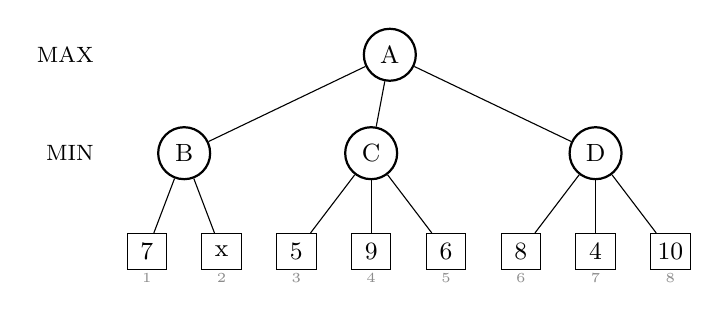
\begin{tikzpicture}[scale=1.0, every node/.style={transform shape}, gc/.style={draw, thick, circle, minimum size=6.6mm, inner sep=0pt, font=\small}, gl/.style={draw, rectangle, minimum width=5mm, minimum height=4.6mm, inner sep=1pt, font=\small}, gx/.style={draw=black!25, text=black!35}, val/.style={font=\footnotesize\bfseries, text=red!80!black, inner sep=1pt}]
\node[font=\footnotesize, anchor=east] at (-0.55,0.00) {MAX};
\node[font=\footnotesize, anchor=east] at (-0.55,-1.25) {MIN};
\node[gc] (n11) at (3.087,0.000) {A};
\node[gc] (n2) at (0.475,-1.250) {B};
\node[gl, label={[font=\tiny, text=black!45, inner sep=1pt]below:1}] (n0) at (0.000,-2.500) {7};
\node[gl, label={[font=\tiny, text=black!45, inner sep=1pt]below:2}] (n1) at (0.950,-2.500) {x};
\node[gc] (n6) at (2.850,-1.250) {C};
\node[gl, label={[font=\tiny, text=black!45, inner sep=1pt]below:3}] (n3) at (1.900,-2.500) {5};
\node[gl, label={[font=\tiny, text=black!45, inner sep=1pt]below:4}] (n4) at (2.850,-2.500) {9};
\node[gl, label={[font=\tiny, text=black!45, inner sep=1pt]below:5}] (n5) at (3.800,-2.500) {6};
\node[gc] (n10) at (5.700,-1.250) {D};
\node[gl, label={[font=\tiny, text=black!45, inner sep=1pt]below:6}] (n7) at (4.750,-2.500) {8};
\node[gl, label={[font=\tiny, text=black!45, inner sep=1pt]below:7}] (n8) at (5.700,-2.500) {4};
\node[gl, label={[font=\tiny, text=black!45, inner sep=1pt]below:8}] (n9) at (6.650,-2.500) {10};
\draw (n11) -- (n2);
\draw (n11) -- (n6);
\draw (n11) -- (n10);
\draw (n2) -- (n0);
\draw (n2) -- (n1);
\draw (n6) -- (n3);
\draw (n6) -- (n4);
\draw (n6) -- (n5);
\draw (n10) -- (n7);
\draw (n10) -- (n8);
\draw (n10) -- (n9);
\end{tikzpicture}
\end{adjustbox}
\end{center}
\subq{(a)}For which values of $x$ are leaves \#4 and \#5 pruned?
\begin{ansbox}[height=1.4cm]\end{ansbox}
\subq{(b)}Is leaf \#8 ever evaluated?
\begin{ansbox}[height=1.2cm]\end{ansbox}
\subq{(c)}Give the root value as a function of $x$ and say for which $x$ MAX chooses B.
\begin{ansbox}[height=1.6cm]\end{ansbox}
\question{6}Consider the expectimax tree below; each chance node has three equally likely outcomes.\begin{center}
\begin{adjustbox}{max width=\linewidth}
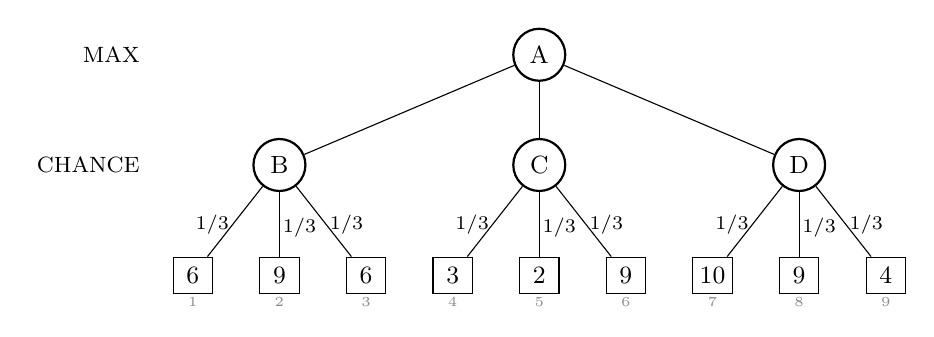
\begin{tikzpicture}[scale=1.0, every node/.style={transform shape}, gc/.style={draw, thick, circle, minimum size=6.6mm, inner sep=0pt, font=\small}, gl/.style={draw, rectangle, minimum width=5mm, minimum height=4.6mm, inner sep=1pt, font=\small}, gx/.style={draw=black!25, text=black!35}, val/.style={font=\footnotesize\bfseries, text=red!80!black, inner sep=1pt}]
\node[font=\footnotesize, anchor=east] at (-0.55,0.00) {MAX};
\node[font=\footnotesize, anchor=east] at (-0.55,-1.40) {CHANCE};
\node[gc] (n12) at (4.400,0.000) {A};
\node[gc] (n3) at (1.100,-1.400) {B};
\node[gl, label={[font=\tiny, text=black!45, inner sep=1pt]below:1}] (n0) at (0.000,-2.800) {6};
\node[gl, label={[font=\tiny, text=black!45, inner sep=1pt]below:2}] (n1) at (1.100,-2.800) {9};
\node[gl, label={[font=\tiny, text=black!45, inner sep=1pt]below:3}] (n2) at (2.200,-2.800) {6};
\node[gc] (n7) at (4.400,-1.400) {C};
\node[gl, label={[font=\tiny, text=black!45, inner sep=1pt]below:4}] (n4) at (3.300,-2.800) {3};
\node[gl, label={[font=\tiny, text=black!45, inner sep=1pt]below:5}] (n5) at (4.400,-2.800) {2};
\node[gl, label={[font=\tiny, text=black!45, inner sep=1pt]below:6}] (n6) at (5.500,-2.800) {9};
\node[gc] (n11) at (7.700,-1.400) {D};
\node[gl, label={[font=\tiny, text=black!45, inner sep=1pt]below:7}] (n8) at (6.600,-2.800) {10};
\node[gl, label={[font=\tiny, text=black!45, inner sep=1pt]below:8}] (n9) at (7.700,-2.800) {9};
\node[gl, label={[font=\tiny, text=black!45, inner sep=1pt]below:9}] (n10) at (8.800,-2.800) {4};
\draw (n12) -- (n3);
\draw (n12) -- (n7);
\draw (n12) -- (n11);
\draw (n3) -- (n0) node[pos=0.55, left, font=\scriptsize, inner sep=1pt]{$1/3$};
\draw (n3) -- (n1) node[pos=0.55, right, font=\scriptsize, inner sep=1pt]{$1/3$};
\draw (n3) -- (n2) node[pos=0.55, right, font=\scriptsize, inner sep=1pt]{$1/3$};
\draw (n7) -- (n4) node[pos=0.55, left, font=\scriptsize, inner sep=1pt]{$1/3$};
\draw (n7) -- (n5) node[pos=0.55, right, font=\scriptsize, inner sep=1pt]{$1/3$};
\draw (n7) -- (n6) node[pos=0.55, right, font=\scriptsize, inner sep=1pt]{$1/3$};
\draw (n11) -- (n8) node[pos=0.55, left, font=\scriptsize, inner sep=1pt]{$1/3$};
\draw (n11) -- (n9) node[pos=0.55, right, font=\scriptsize, inner sep=1pt]{$1/3$};
\draw (n11) -- (n10) node[pos=0.55, right, font=\scriptsize, inner sep=1pt]{$1/3$};
\end{tikzpicture}
\end{adjustbox}
\end{center}
\subq{(a)}Calculate the expectimax value of every node.
\begin{ansbox}[height=1.4cm]\end{ansbox}
\subq{(b)}Now assume every leaf value is at most 10 (and at least 0). Evaluating leaves left to right, identify the branches that can be pruned and explain each.
\begin{ansbox}[height=2.0cm]\end{ansbox}
\clearpage
\question{7}Rollouts return 1 (win), 0.5 (draw) or 0 (loss) for the root player. Use $\mathrm{UCB1}=\bar V_i+C\sqrt{\ln N/n_i}$ (unvisited $=\infty$, ties to the left; a never-visited leaf is rolled out directly, otherwise all its children are added and the rollout starts at the first; $X_1\to X_3,X_4$ and $X_2\to X_5,X_6$ for $X\in\{A,B,C\}$). The current tree is:\begin{center}
\begin{adjustbox}{max width=\linewidth}
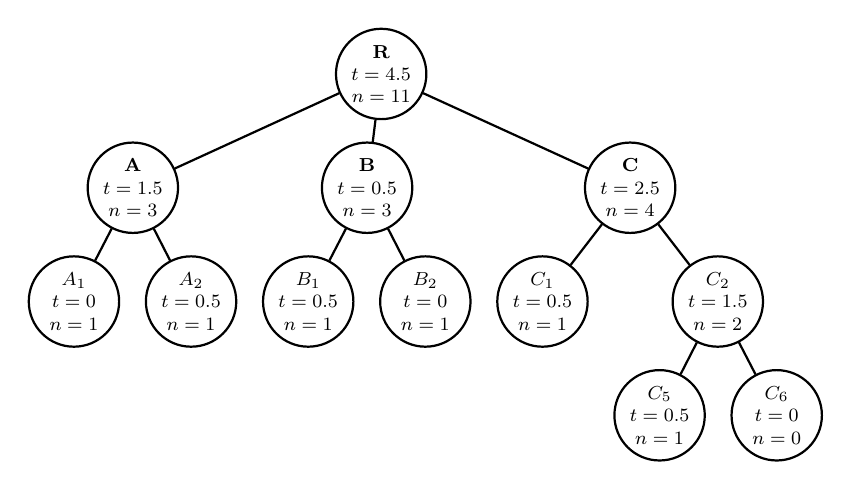
\begin{tikzpicture}[scale=0.85, every node/.style={transform shape}, mn/.style={draw, thick, circle, align=center, font=\footnotesize, inner sep=0.5pt, minimum size=13.5mm}]
\node[mn] (m1) at (4.59,0.00) {\textbf{R}\\ $t=4.5$\\ $n=11$};
\node[mn] (m2) at (0.88,-1.70) {\textbf{A}\\ $t=1.5$\\ $n=3$};
\node[mn] (m3) at (0.00,-3.40) {\textbf{$A_{1}$}\\ $t=0$\\ $n=1$};
\draw[thick] (m2) -- (m3);
\node[mn] (m4) at (1.75,-3.40) {\textbf{$A_{2}$}\\ $t=0.5$\\ $n=1$};
\draw[thick] (m2) -- (m4);
\draw[thick] (m1) -- (m2);
\node[mn] (m5) at (4.38,-1.70) {\textbf{B}\\ $t=0.5$\\ $n=3$};
\node[mn] (m6) at (3.50,-3.40) {\textbf{$B_{1}$}\\ $t=0.5$\\ $n=1$};
\draw[thick] (m5) -- (m6);
\node[mn] (m7) at (5.25,-3.40) {\textbf{$B_{2}$}\\ $t=0$\\ $n=1$};
\draw[thick] (m5) -- (m7);
\draw[thick] (m1) -- (m5);
\node[mn] (m8) at (8.31,-1.70) {\textbf{C}\\ $t=2.5$\\ $n=4$};
\node[mn] (m9) at (7.00,-3.40) {\textbf{$C_{1}$}\\ $t=0.5$\\ $n=1$};
\draw[thick] (m8) -- (m9);
\node[mn] (m10) at (9.62,-3.40) {\textbf{$C_{2}$}\\ $t=1.5$\\ $n=2$};
\node[mn] (m11) at (8.75,-5.10) {\textbf{$C_{5}$}\\ $t=0.5$\\ $n=1$};
\draw[thick] (m10) -- (m11);
\node[mn] (m12) at (10.50,-5.10) {\textbf{$C_{6}$}\\ $t=0$\\ $n=0$};
\draw[thick] (m10) -- (m12);
\draw[thick] (m8) -- (m10);
\draw[thick] (m1) -- (m8);
\end{tikzpicture}
\end{adjustbox}
\end{center}
\subq{(a)}With $C=\sqrt2$, calculate UCB1 of $A$, $B$, $C$. Which child is selected? For which values of $C$ would the root select $C$ instead of $A$?
\begin{ansbox}[height=2.4cm]\end{ansbox}
\subq{(b)}Perform three iterations whose rollouts return $0,\ 0.5,\ 0$ (in order); update the statistics and draw the final tree.
\begin{ansbox}[height=8.0cm]\end{ansbox}
\clearpage
\question{8}This problem is about map colouring. Each region must be coloured Red (R), Green (G) or Blue (B), and neighbouring regions must have different colours. The constraint graph is shown below. The following questions are mutually independent.\begin{center}
\begin{adjustbox}{max width=\linewidth}
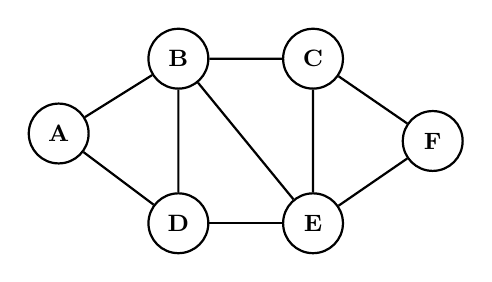
\begin{tikzpicture}[scale=0.95, every node/.style={transform shape}, cv/.style={draw, thick, circle, minimum size=8mm, inner sep=0pt, font=\small\bfseries}]
\node[cv] (A) at (0.00,1.20) {A};
\node[cv] (B) at (1.60,2.20) {B};
\node[cv] (C) at (3.40,2.20) {C};
\node[cv] (D) at (1.60,0.00) {D};
\node[cv] (E) at (3.40,0.00) {E};
\node[cv] (F) at (5.00,1.10) {F};
\draw[thick] (A) to[] (B);
\draw[thick] (A) to[] (D);
\draw[thick] (B) to[] (C);
\draw[thick] (B) to[] (D);
\draw[thick] (B) to[] (E);
\draw[thick] (C) to[] (E);
\draw[thick] (C) to[] (F);
\draw[thick] (D) to[] (E);
\draw[thick] (E) to[] (F);
\end{tikzpicture}
\end{adjustbox}
\end{center}
\subq{(a)}\textbf{Cross out} all values that would be eliminated by \emph{forward checking} after variable B has been assigned as shown.\begin{center}\small\begin{tabular}{|l|c|c|c|c|c|c|}\hline Variables & \textbf{A} & \textbf{B} & \textbf{C} & \textbf{D} & \textbf{E} & \textbf{F}\\ \hline Domains & R\ G\ B & \textbf{R} & R\ G\ B & R\ G\ B & R\ G\ B & R\ G\ B\\ \hline\end{tabular}\end{center}

\subq{(b)}A and B have been assigned as shown, but no constraint propagation has been done yet. \textbf{Cross out} all values that would be eliminated by \emph{arc consistency} (AC-3).\begin{center}\small\begin{tabular}{|l|c|c|c|c|c|c|}\hline Variables & \textbf{A} & \textbf{B} & \textbf{C} & \textbf{D} & \textbf{E} & \textbf{F}\\ \hline Domains & \textbf{R} & \textbf{G} & R\ G\ B & R\ G\ B & R\ G\ B & R\ G\ B\\ \hline\end{tabular}\end{center}

\subq{(c)}Variable A is already assigned and constraint propagation has been done. \textbf{Circle} all unassigned variables that might be selected by the \emph{Minimum-Remaining-Values} (MRV) heuristic.\begin{center}\small\begin{tabular}{|l|c|c|c|c|c|c|}\hline Variables & \textbf{A} & \textbf{B} & \textbf{C} & \textbf{D} & \textbf{E} & \textbf{F}\\ \hline Domains & \textbf{R} & G\ B & R\ G\ B & G\ B & R\ G\ B & R\ G\ B\\ \hline\end{tabular}\end{center}

\subq{(d)}Same situation. \textbf{Circle} all unassigned variables that might be selected by the \emph{Degree Heuristic}.\begin{center}\small\begin{tabular}{|l|c|c|c|c|c|c|}\hline Variables & \textbf{A} & \textbf{B} & \textbf{C} & \textbf{D} & \textbf{E} & \textbf{F}\\ \hline Domains & \textbf{R} & G\ B & R\ G\ B & G\ B & R\ G\ B & R\ G\ B\\ \hline\end{tabular}\end{center}

\subq{(e)}Assume no variable has been assigned yet. Solve the CSP using backtracking with \emph{forward checking}, choosing variables with MRV, then the degree heuristic (DH), and finally alphabetical order; try values in the order R, G, B. For every step give the MRV value of every region not yet coloured, and the DH values of the regions tied on the minimum MRV.
\par \underline{Step 1}\par\begin{center}\small \begin{tabular}{|l|c|c|c|c|c|c|}\hline Variables & \textbf{A} & \textbf{B} & \textbf{C} & \textbf{D} & \textbf{E} & \textbf{F}\\ \hline MRV & \phantom{0} & \phantom{0} & \phantom{0} & \phantom{0} & \phantom{0} & \phantom{0}\\[1mm]\hline DH & \phantom{0} & \phantom{0} & \phantom{0} & \phantom{0} & \phantom{0} & \phantom{0}\\[1mm]\hline\end{tabular}\end{center}Assign to the variable \rule{2.5cm}{0.3pt} with the value \rule{2.5cm}{0.3pt}\par
\underline{Step 2}\par\begin{center}\small \begin{tabular}{|l|c|c|c|c|c|c|}\hline Variables & \textbf{A} & \textbf{B} & \textbf{C} & \textbf{D} & \textbf{E} & \textbf{F}\\ \hline MRV & \phantom{0} & \phantom{0} & \phantom{0} & \phantom{0} & \phantom{0} & \phantom{0}\\[1mm]\hline DH & \phantom{0} & \phantom{0} & \phantom{0} & \phantom{0} & \phantom{0} & \phantom{0}\\[1mm]\hline\end{tabular}\end{center}Assign to the variable \rule{2.5cm}{0.3pt} with the value \rule{2.5cm}{0.3pt}\par
\underline{Step 3}\par\begin{center}\small \begin{tabular}{|l|c|c|c|c|c|c|}\hline Variables & \textbf{A} & \textbf{B} & \textbf{C} & \textbf{D} & \textbf{E} & \textbf{F}\\ \hline MRV & \phantom{0} & \phantom{0} & \phantom{0} & \phantom{0} & \phantom{0} & \phantom{0}\\[1mm]\hline DH & \phantom{0} & \phantom{0} & \phantom{0} & \phantom{0} & \phantom{0} & \phantom{0}\\[1mm]\hline\end{tabular}\end{center}Assign to the variable \rule{2.5cm}{0.3pt} with the value \rule{2.5cm}{0.3pt}\par
\underline{Step 4}\par\begin{center}\small \begin{tabular}{|l|c|c|c|c|c|c|}\hline Variables & \textbf{A} & \textbf{B} & \textbf{C} & \textbf{D} & \textbf{E} & \textbf{F}\\ \hline MRV & \phantom{0} & \phantom{0} & \phantom{0} & \phantom{0} & \phantom{0} & \phantom{0}\\[1mm]\hline DH & \phantom{0} & \phantom{0} & \phantom{0} & \phantom{0} & \phantom{0} & \phantom{0}\\[1mm]\hline\end{tabular}\end{center}Assign to the variable \rule{2.5cm}{0.3pt} with the value \rule{2.5cm}{0.3pt}\par
\underline{Step 5}\par\begin{center}\small \begin{tabular}{|l|c|c|c|c|c|c|}\hline Variables & \textbf{A} & \textbf{B} & \textbf{C} & \textbf{D} & \textbf{E} & \textbf{F}\\ \hline MRV & \phantom{0} & \phantom{0} & \phantom{0} & \phantom{0} & \phantom{0} & \phantom{0}\\[1mm]\hline DH & \phantom{0} & \phantom{0} & \phantom{0} & \phantom{0} & \phantom{0} & \phantom{0}\\[1mm]\hline\end{tabular}\end{center}Assign to the variable \rule{2.5cm}{0.3pt} with the value \rule{2.5cm}{0.3pt}\par
\underline{Step 6}\par Assign to the variable \rule{2.5cm}{0.3pt} with the value \rule{2.5cm}{0.3pt}\par
\clearpage
\question{9}Cryptarithmetic: $\;\begin{array}{r} T\,O\\ +\;G\,O\\ \hline O\,U\,T\end{array}\;$ --- distinct letters are distinct digits and leading digits are non-zero.
\subq{(a)}Formulate the CSP: variables (including carries), domains and constraints.
\begin{ansbox}[height=2.0cm]\end{ansbox}
\subq{(b)}Solve it by constraint propagation, explaining each deduction.
\begin{ansbox}[height=2.4cm]\end{ansbox}
\question{10}\textit{Lab scheduling.} Five lab sessions must each be run by one TA, and a TA cannot run two overlapping sessions: P1 8:00--9:30, P2 9:00--10:30, P3 9:30--11:00, P4 10:30--12:00, P5 11:30--13:00 (sessions that only touch do not overlap). TA \textbf{H} can run P1, P2, P4, P5; \textbf{L} can run P2, P3; \textbf{M} can run P1, P3, P4.
\subq{(a)}Formulate the CSP (one variable per session; apply the availability constraints to the domains) and draw the constraint graph.
\begin{center}\small\begin{tabular}{|l|c|c|c|c|c|}\hline Variables & \textbf{P1} & \textbf{P2} & \textbf{P3} & \textbf{P4} & \textbf{P5}\\ \hline Domains &  &  &  &  & \\ \hline\end{tabular}\end{center}\begin{ansbox}[height=2.4cm]\end{ansbox}
\subq{(b)}Run AC-3 with the initial queue $P1\to P2$, $P2\to P1$, $P2\to P3$, $P3\to P2$, $P3\to P4$, $P4\to P3$, $P4\to P5$, $P5\to P4$. Cross out the values it eliminates from your domains in (a), and give the solution.
\begin{ansbox}[height=5.0cm]\end{ansbox}
\clearpage
\question{11}Answer the following questions briefly.
\subq{(a)}Match each field with its contribution to AI: (1) Philosophy, (2) Mathematics, (3) Economics, (4) Neuroscience, (5) Psychology, (6) Control theory. (a) neurons as information-processing units; (b) utility and decision theory; (c) logic, reasoning, mind as a physical system; (d) maximising an objective function over time; (e) formal proof, algorithms, (in)tractability, probability; (f) how people perceive, process information and represent knowledge.
\begin{ansbox}[height=1.0cm]\end{ansbox}
\subq{(b)}Order chronologically and explain the AI winter: Deep Blue beats Kasparov; Dartmouth meeting; McCulloch \& Pitts; AlphaGo beats Lee Sedol; Turing's ``Computing Machinery and Intelligence''; the expert-systems boom.
\begin{ansbox}[height=2.0cm]\end{ansbox}
\subq{(c)}For the 8-puzzle below compute $h_1$ (misplaced tiles) and $h_2$ (total Manhattan distance). Which heuristic dominates the other, and what does dominance imply for A*?\par\begin{center}Start: {\renewcommand{\arraystretch}{1.3}\begin{tabular}{|c|c|c|}\hline 4 & 1 & 2 \\ \hline
 & 8 & 7 \\ \hline
6 & 3 & 5 \\ \hline\end{tabular}}\qquad Goal: {\renewcommand{\arraystretch}{1.3}\begin{tabular}{|c|c|c|}\hline  & 1 & 2 \\ \hline
3 & 4 & 5 \\ \hline
6 & 7 & 8 \\ \hline\end{tabular}}\end{center}
\begin{ansbox}[height=2.4cm]\end{ansbox}
\subq{(d)}A CSP has $n=5$ variables with domain size $d=3$. How many leaves does a naive search tree (any unassigned variable at each level) have, and how many with backtracking? Which property justifies the difference?
\begin{ansbox}[height=2.0cm]\end{ansbox}
\question{12}True or false?
For each statement, circle \textbf{T} or \textbf{F} and justify your answer in one or two sentences (an answer without a correct justification earns no credit).
\subq{1.}Uniform-cost search expands nodes in order of their optimal path cost. \hfill \textbf{T \quad F}
\begin{ansbox}[height=1.5cm]\end{ansbox}
\subq{2.}A* is optimally efficient among optimal algorithms using the same heuristic. \hfill \textbf{T \quad F}
\begin{ansbox}[height=1.5cm]\end{ansbox}
\subq{3.}If $h(n)=0$ for every node, A* behaves exactly like UCS. \hfill \textbf{T \quad F}
\begin{ansbox}[height=1.5cm]\end{ansbox}
\subq{4.}If $h_2$ dominates $h_1$ and both are consistent, A* with $h_2$ never expands more nodes than A* with $h_1$ (ignoring ties). \hfill \textbf{T \quad F}
\begin{ansbox}[height=1.5cm]\end{ansbox}
\subq{5.}Local beam search with $k$ states is the same as $k$ independent random-restart hill climbs run in parallel. \hfill \textbf{T \quad F}
\begin{ansbox}[height=1.5cm]\end{ansbox}
\subq{6.}The amount of alpha-beta pruning does not depend on the move ordering. \hfill \textbf{T \quad F}
\begin{ansbox}[height=1.5cm]\end{ansbox}
\subq{7.}Against a sub-optimal MIN player, the minimax move always gives MAX the best possible outcome. \hfill \textbf{T \quad F}
\begin{ansbox}[height=1.5cm]\end{ansbox}
\subq{8.}MCTS grows its tree symmetrically, level by level. \hfill \textbf{T \quad F}
\begin{ansbox}[height=1.5cm]\end{ansbox}
\subq{9.}Node consistency concerns binary constraints. \hfill \textbf{T \quad F}
\begin{ansbox}[height=1.5cm]\end{ansbox}
\subq{10.}The degree heuristic is mainly used as a tie-breaker for MRV. \hfill \textbf{T \quad F}
\begin{ansbox}[height=1.5cm]\end{ansbox}
\end{document}